% !TeX root = ../main.tex

\chapter{ROS上的机器人导航算法}

\section{ROS导航}

ROS(Robot Operating System)是一个开源的专用于机器人软件开发的操作系统。ROS中提供了一个模块化的简单2D导航系统ROS Navigation,其主要架构如图\ref{fig:rosnav}所示。在已有的导航结构的基础上,我们可以以插件的形式添加所需的行人识别和追踪模块,并根据此信息和用户的要求进行行人跟随。

\begin{figure}[htb]
  \centering
  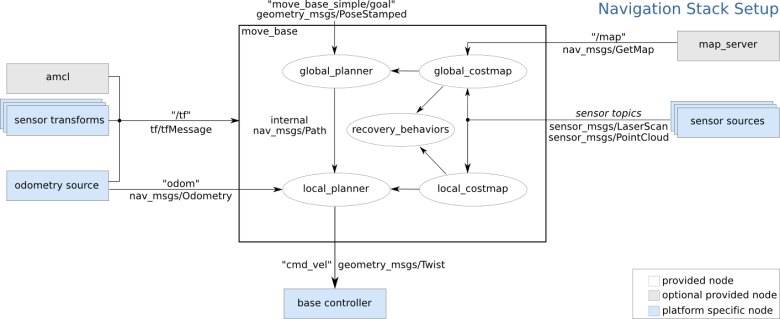
\includegraphics[width=1.1\textwidth]{ROS_navigation_stack.png}
  \caption{ROS导航架构}
  \label{fig:rosnav}
\end{figure}

\subsection{坐标系转换}
  在机器人系统中存在数个坐标系,包括机器人底座为中心的坐标系,2D激光传感器为中心的坐标系,摄像机为中心的坐标系,全局地图上的坐标系等。为了能使各个传感器得到的不同坐标系下的信息方便准确地结合使用,ROS导航提供了tf系统,由用户指定不同坐标系之间的tf变换,并存储起来,维护一个tf变换树。在调用tf变换时,只需要指定原坐标系的结点和需要变换的目标坐标系的节点,tf系统就会自动计算出两个坐标系之间的相对位置和角度,并完成坐标的转换。

\subsection{里程计}
  机器人的里程计包括机器人的位姿(pose)和速度(twist),其中,机器人的位姿和其姿势,可以由机器人的初始位置和机器人的控制单元的速度,通过运动模型计算得到的,也可以通过激光扫描数据对机器人位置的定位得到。里程计信息并被发布给局部规划器,用于路径规划。

\subsection{建图}
  对于有里程计和固定水平激光测距仪的机器人,在地面平坦的情况下,可以使用gmapping\cite{grisetti2007improved}的方式进行建图。此外还可以选择cartographer\cite{hess2016real}方法,在没有里程计,激光测距仪不是完全水平的情况下,如使用者手持激光测距仪的情况下也可以进行建图。建图是实时的,即把当前激光扫描到的物体根据当前的定位加入地图中,所以在室内环境下时,在使用前首先操作机器人将室内环境扫描一遍,即可建立室内的地图。地图使用一个描述地图元数据的YAML文件和一个编码了图中占用/自由点的image文件存储起来,ROS导航中提供一个map\_server节点用于发布地图数据。

  由于地图是静态存储的,而环境通常是动态的,为了应对机器人实际运行中可能遇到的意想不到的动态障碍,还需要维护代价地图(costmap)。代价地图采用传感器数据和来自静态地图的信息,以一定的频率进行更新,来存储和掌握实际环境中的障碍物信息。在ROS导航中,维护两个代价地图,分别用于在整个环境上的全局和长期规划,以及局部区域内的规划和避障。

\subsection{定位}
  自适应蒙特卡罗定位(adaptive Monte Carlo localization,amcl)模块是机器人的定位模块,在建立地图后使用,使用粒子滤波算法进行对机器人当前位置的估计。通过在图上均匀地撒上一些点,再随着机器人在图中的运动,计算每个点的机器人当前位置的概率,减少概率小的位置点的密度,增加概率大的位置点的密度,在粒子不断收敛后即可较为准确地得到机器人在图中的位置。

\subsection{导航控制}

  导航控制模块即图\ref{fig:rosnav}中的move\_base模块,包括全局规划器、局部规划器和恢复机制。全局导航支持${\rm A}^\ast$算法和dijkstra算法来在全局代价地图上找到前往下一个目的地的最短路径,在机器人开始移动之前就首先被计算出来。局部规划器监控了传感器信息,结合了里程计信息、全局和局部代价地图来选择机器人在全局路径的局部分块中应选择的最佳速度(线速度和角速度),传送给base\_control模块。同时,局部规划器也可以动态地重新规划机器人的局部路径以进行避障,使用动态窗口法(Dynamic Window)\cite{fox1997dynamic}进行局部避障,使用路径展开法(Trajectory Rollout)\cite{gerkey2008planning}进行局部规划和控制。恢复机制用于出现了异常情况,机器人无法进行决策时使用,ROS导航提供了两种恢复行为,使用静态地图在用户指定的更大范围外恢复代价地图,或通过使机器人$360^{\circ}$旋转来尝试清出空间。

\section{可佳导航}

\begin{figure}[htb]
  \centering
  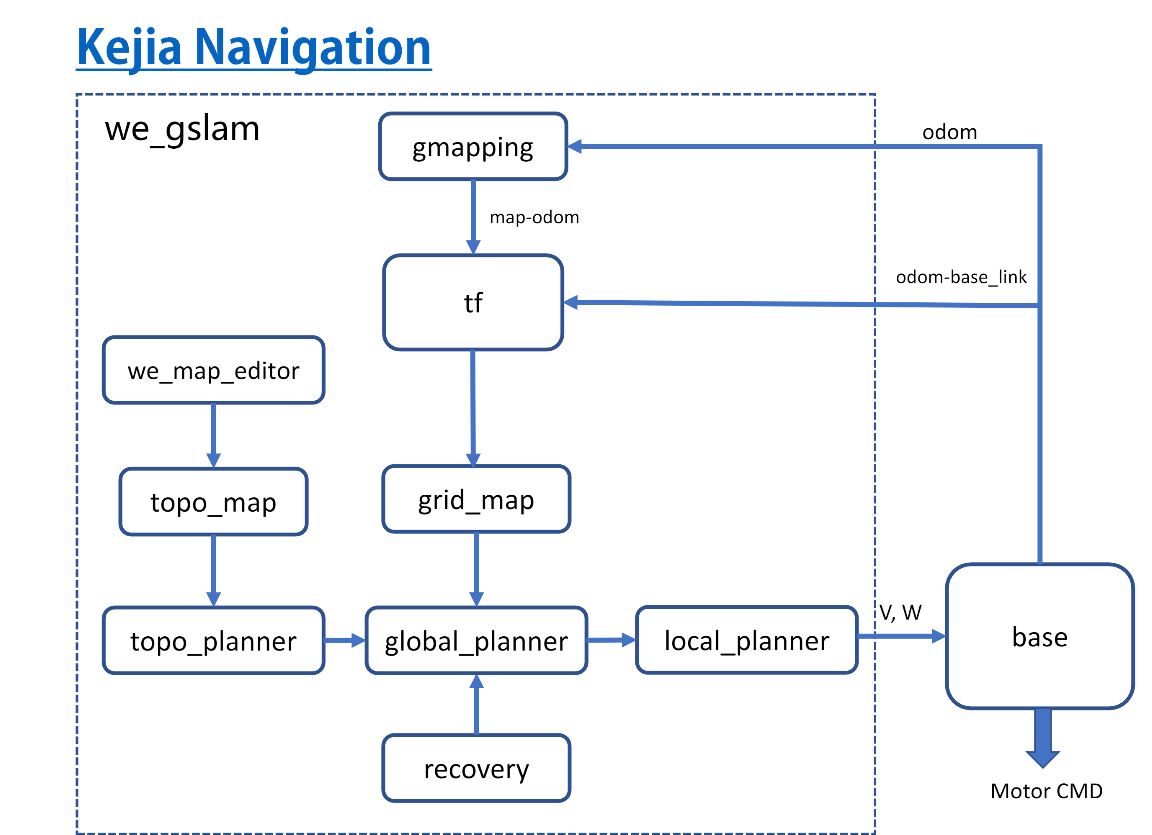
\includegraphics[width=0.8\textwidth]{kejianav.png}
  \caption{可佳导航架构}
  \label{fig:kejianav}
\end{figure}

  可佳导航的架构如图\ref{fig:kejianav}所示,它同样使用ROS系统用于软件的运行和各模块之间的通信。在导航方面,它相对于ROS导航,还加入了拓扑导航和语义地图。通过手动注释如房间、门、家具等对象的大致位置和区域,自动生成一个拓扑地图,该拓扑地图会用于全局路径规划和定位。

  可佳导航使用${\rm A}^\ast$算法进行全局和局部的路径规划,并使用向量场直方图(vector field histogram,VFH)\cite{borenstein1991vector}进行局部避障。可佳导航使用了一个状态机来进行任务的规划和决策。在收到任务目标后,它首先在全局地图上运行${\rm A}^\ast$算法,并将全局路径分成一些局部目的地(waypoints),将最近的waypoint作为VFH算法的目标点,运行局部的避障。如果遇到了障碍物,将障碍物更新到本地代价地图中,重新运行${\rm A}^\ast$的局部路径规划,如果此处的局部路径规划失败,则运行恢复机制\cite{liu2017wrighteagle}。
